%
\section{Introduction}

Vulnerability testing attempts to identify weaknesses in code
that could ultimately lead to exploits capable of compromising
computing systems. Attempts to automate vulnerability testing can
potentially take many forms. For example, Kayac\i{}k et al.,
proposed a framework in which a genetic program was rewarded for
finding `Smash the Stack' style shellcode attacks which
simultaneously minimized IDS alarm rates
\cite{kayacik06,kayacik11}. However, such attacks are only viable
as long as stack (i.e., writable) memory is mapped as an
executable. An attempt to redirect the instruction pointer to
non-executeable memory will result in a relatively harmless
segfault.\footnote{Still of concern as a potential DoS vector,
but this is nowhere near as serious as the threat of arbitrary
code execution.} Non-executable stacks, however, are today the
rule rather than the exception, thanks to security features
supported by most compilers (e.g.\ both \textsc{gcc} and \textsc{clang} provide this
feature).

Mechanisms for circumnavigating the obstacle of non-executable stacks were demonstrated as early as 1997 when `Solar Designer' posted the return-into-libc technique to the
Bugtraq mailing
list.\footnote{\url{http://seclists.org/bugtraq/1997/Aug/63}}
Unlike traditional shellcode attacks, where the attacker places
executable code onto the stack (either in an input buffer or an
environment variable, for instance) and then redirects the
instruction pointer to that code, Solar Designer�s attack simply
uses code that is already mapped to executable memory. Since libc
is almost always going to be resident in the executable memory of
a Unix process, it makes for a convenient target. Thus,
conceptually at least, all that is necessary is to redirect the
instruction pointer to, say, the \texttt{system()} function, with
the desired parameters, such as a pointer to the string
\texttt{/bin/sh}. This works because libc contains procedures
useful to a potential attacker, such as code fragments for
performing system calls. The attacker need not write any more
code, just over-write the return address of a library function,
continuing the process for additional stack locations. The trick
is to make sure that the return addresses collectively describe a
new function by selectively targeting appropriate library
functions.% The matter is somewhat more complicated when dealing
with more modern ABIs, such as \textsc{arm} and x86\_64, where the first
few function arguments are passed in registers.

Return-oriented-programming (\textsc{rop}) is a generalization of this
technique. Instead of redirecting execution to already resident
functions, \textsc{rop} targets a far more general class of instruction
sequences. Specifically, new arbitrary programmes are constructed
from \textit{scraps} of code sequences available in executable
memory (or `gadgets'). The goal of the attacker is to assemble
the gadgets into complex chains through judicious use of gadget
return addresses, thus describing new arbitrary programmes. This
was first demonstrated on the x86 \cite{shacham07} and then the
\textsc{risc} architecture \cite{buchanan08}. More recently, an approach
to \textsc{rop} under x86 and \textsc{arm} architectures was identified without
using the return instruction \cite{checkoway10}, i.e.\ instruction
sequences are identified that collectively mimic the return
instruction; thus making detection more difficult.

This work introduces \textsc{Roper}, a genetic compiler that evolves payloads for
return-oriented programming (\textsc{rop}) attacks.%
\footnote{\url{https://github.com/oblivia-simplex/roper}}
These are
attacks that manipulate their host's control flow in subtle and
fine-grained ways, and, unlike traditional shellcode attacks,
they do this without at any point introducing foreign code,
or writing to executable memory. Since it is becoming
increasingly rare for processes to map \emph{any} segment of
memory as both writeable and executable -- due to a defensive
measure called `Data Execution Prevention' (\textsc{dep}) when
implemented on Windows, or `Write xor Execute'
%% mention also harvard bus architectures, etc. 
($W \oplus X$), when implemented in a Unix environment --
return-oriented programming (or \textsc{rop}) has become the
industry standard approach to payloads in binary exploit
development. 

\textsc{rop} works by sifting through the host process's executable memory
-- its \texttt{.text} segment, in the case of \textsc{elf} binaries -- and search for chunks of code that can be
rearranged in such a way that they carry out the attacker's
wishes, rather than their intended design. For these chunks to be
usable in an attack, however, it must be possible to jump from
one to the other in a predetermined sequence. This is where the
`return-oriented' nature of the attack comes in: most
architectures implement subroutine or function calls by first
pushing the address of the instruction \emph{after} the call to
the stack, and then jump to the first instruction of a
subroutine that, itself, ends by popping the bookmarked `return
address' from the stack. In a \textsc{rop} attack, we exploit
this manner of implementing returns. We set things up so that
the `return address' popped from the stack at the end of each
`gadget' is just a pointer to the next gadget we wish to execute.
This lets us chain together multiple \textsc{rop}
gadgets in sequence. In principle, it is possible to
implement complex attacks in this fashion, without ever needing
to use any executable code that is not already there, waiting for
us in the process's executable memory segment (\S~\ref{sec:RopBackgnd} summarizes recent \textsc{rop} code bases).

These chains are the kind of entities that our engine evolves
(\S~\ref{sec:methodology}). The genetic material consists of
the set of gadgets extracted from a target executable binary --
we focus for now on \textsc{elf} binaries compiled for 32-bit
\textsc{arm} processors. The individual genotypes are
\textsc{rop}-chains, formed from this material. The phenotype, on
which selection pressures are brought to bear, is the behaviour
these genotypes exhibit when executed in a virtual (but
realistic) \textsc{cpu}. The entire set up resembles a variation
on linear genetic programming, but with a few key differences,
required by the nature of the problem at hand. The goal is to not
simply automate the tricky and time-consuming human task
of assembling \textsc{rop}-chain payloads -- though
\textsc{roper} does that quite well -- but to explore an entirely
novel class of payloads: \textsc{rop}-chains that exhibit the
sort of subtle and adaptive behaviour for which we normally turn
to machine learning. 

As a proof of concept, we evolve \textsc{rop}-chain payloads that
cannibalize arbitrary binaries into mosaics capable of solving a
traditional benchmark classification problem, specifically with
the famous Iris dataset (\S~\ref{sec:empirical}). Without
injecting a single foreign instruction, we will coax system and
backend binaries into tasks that resemble nothing they were
designed to do, and nothing that has previously been attempted in
low-level binary exploitation: in short, \textsc{Roper} will sort
flowers. Section~\ref{sec:conclude} concludes the paper and
identifies future work.

\section{Related Work}\label{sec:RopBackgnd}


%\subsection{Return-Oriented Programming}

%\subsection{Linear Genetic Programming}
% maybe move that other bit up here
%\subsection{Prior Research and Development}

% Stephanie Forrest
% Bill Langdon (sp?) (UK)

%\subsubsection{ROP-Chain Compilers}

A handful of technologies have already been developed for the
automatic generation of \textsc{rop}-chains. These range from
tools that use one of several determinate recipes for assembling
a chain -- such as the {Corelan Team}'s extraordinarily useful
\texttt{mona.py} -- to tools\footnote{\url{https://github.com/corelan/mona}} which approach the problem through
the lens of compiler design, grasping the set of gadgets
extracted from a binary as the instruction set of a baroque and
supervenient virtual machine. %% Maybe add a quote or two. 

We are aware of two such projects at the moment. The first, named
\emph{Q} \cite{shacham07}. The second, \textsc{ropc}, grew out of
its authors' attempts to reverse engineer $Q$, and extend its
capabilities to the point where it could compile
\textsc{rop}-chains for scripts written in a Turing-complete
programming language.%
\footnote{\url{https://github.com/pakt/ropc}} This latter project
has since inspired a fork that aims to use \textsc{ropc}'s own
intermediate language as an \textsc{llvm} backend, which, if
successful, would let programmes written in any language that
compiles to \textsc{llvm}'s intermediate language, compile to
\textsc{ropc}-generated \textsc{rop}-chains as well.  

Another, particularly interesting contribution in the field of
automated \textsc{rop}-chain generation is \emph{Braille}, which
automates an attack that its developers term ``Blind
Return-Oriented Programming", or \textsc{brop} \cite{bittau14}.
\textsc{brop} solves the problem of developing \textsc{rop}-chain
attacks against processes where not only the source code but the
binary itself in unknown. %% Perhaps add more details
\emph{Braille} first uses a stack-reading technique to probe a
vulnerable process (one that is subject to a buffer overflow and
which automatically restarts after crashing), to find enough
gadgets, through trial and error, for a simple \textsc{rop} chain
whose purpose will be to write the process's executable memory
segment to a socket, sending that segment's data back to the
attacker -- data that is then used, in conjunction with address
information obtained through stack-reading, to construct a more
elaborate \textsc{rop}-chain the old-fashioned way. It is an
extremely interesting and clever technique, which could, perhaps,
be fruitfully combined with the genetic techniques we will
outline here. 

To the best of our knowledge, neither evolutionary nor other
machine-learning-driven techniques have been employed in the
generation of \textsc{rop} attacks. Such techniques \emph{have},
however, been put to use in order to defend against such attacks.
The development of the HadROP detection system, by Pfaff et
al., represents a recent contribution to this field \cite{pfaff15}, training support
vector machines on the behaviour of hardware performance
counters, to detect the control flow patterns that are
characteristic of \textsc{rop} attacks.  

\section{Methodology}\label{sec:methodology}

\textsc{Roper} is a complete system for the automatic evolution
of \textsc{rop}-chains meeting a user-supplied specification, and
targetting a given executable. A bird's eye view of the system
can be found in figure~\ref{fig:architecture}. The executable
binary (box 1) supplies the raw material from which a collection
of gadgets is extracted (box 2), and is mapped into the memory
of a virtual machine (box 5). Together with a set of constants
(parsed out of user-supplied input or randomly generated), these
gadgets make up the gene pool from which an initial, random
population will be initialized. This brings us to the genetic
process that forms the core of the system (box 4). The
individuals' genotypes -- sequences of pointers into the
executable (1), which now exists in the memory of the VM (5) --
are sent over to the VM to be mapped into their corresponding
phenotypes. Their behaviour in the \textsc{cpu} and the
resulting \textsc{cpu} context array is returned to the
genetic process (4) to be passed to the fitness functions.  The
fitness functions assess the phenotype images returning to (4)
from (5), together with any information coming from the user (box 3:
labelled data or other specifications). These determine the
process of parent selection (a steady state tournament), after which the
reproduction and variation functions go to work (all of this
takes place in box 4 of our map). The cycle then repeats, with an
ongoing exchange of genotypes for phenotypes between (4) and (5),
until the completion criteria have been reached. 

\begin{figure}
  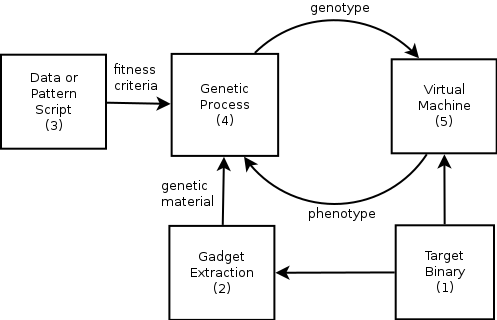
\includegraphics[width=\columnwidth]{architecture.png}
  \caption{High-level map of ROPER's architecture}
  \label{fig:architecture}
\end{figure}

\subsection{Genotype Representation}


\subsubsection{Gadgets, Clumps, and Chains}

Individuals, here, are essentially vectors of 32-bit words, which
may be either pointers into executable memory addresses, intended
to be popped into the program counter, or other values, intended
to be popped into the \textsc{cpu}'s other registers. 

Returns, in \textsc{arm} machine code, are frequently implemented as
multi-pop instructions -- which pop an address from the stack
while simultaneously popping a variable number of additional
words into the other registers. Depending on the target problem, the range of values that could potentially be
made use of in the general purpose registers might be very
different from the range of values where we find pointers into
executable memory. Thus, it makes sense to interleaf address
pointers and other values in a controlled fashion, when
constructing our initial population. 
% also other pops

To do this, we calculate the distance the stack pointer will shift
when each gadget executes, $\Delta_{SP}(g)$, and then clump
together each gadget pointer $g$ with a vector of
$\Delta_{SP}(g)-1$ non-gadget values.%
\footnote{The pop instruction, \texttt{LDMIA! sp, \{r0, r7, 
  r9, pc\}},
  for example, has an $\Delta_{SP}$ of 4. If it's the only
  instruction that moves the stack pointer in gadget $g$, then
  $\Delta_{SP}(g) = 4$, and we will append 3 words to the clump
  that begins with a pointer to $g$.}
These values will populate
the \textsc{cpu}'s registers when the final, multipop instruction of the
gadget is executed. The program counter (\texttt{PC}) is always
the final register populated through a multipop, and so the
address of the next gadget $g'$ should be found exactly
$\Delta_{SP}(g)$ slots up from $g$.%
\footnote{\textsc{rop}ER also handles gadgets that end in a different
  form of return: a pair of instructions that populates a series
  of registers from the stack, followed by an instruction that
  copies that address from one of those registers to \texttt{PC}.
  In these instances, $\Delta{SP}(g)$ and the offset of the next
  gadget from $g$ are distinct. But this is a complication that
  we don't need to dwell on here.}

\subsubsection{Variation Operators}
\paragraph{Mutation}
Structuring the basic units of our genotypes in this way also
lets us apply variation operators more intelligently. The
genotype is much more tolerant of mutations to the non-gadget
values in each clump than to the gadget address itself. The
gadget address \emph{may} be safe to increment or decrement by a
word or two, but negating, multiplying, or masking it would
almost certainly result in a crash. The rest of the words in the
clump can be mutated much more freely, either arithmetically, or
by indirection/dereference (we can replace a value with a pointer
to that value, if one is available, or if a value can already be
read as a valid pointer, we can replace it with its referent).

\paragraph{Crossover}
Our second variation operator is single-point crossover, which
operates at the level of `clumps', not words. We chose
single-point crossover over two-point or uniform crossover
% check terminology
to favour the most likely form gene linkage would take in this
context. A single \textsc{rop}-gadget can transform the \textsc{cpu} context in
fairly complex ways, and, combined with multipop instructions,
the odds that the work performed by a gadget $g$ will be
clobbered by a subsequent gadget $g'$ increases greatly with the
distance of $g'$ from $g$. This means that adjacent gadgets are
more likely to achieve a combined, fitness-relevant effect, than
non-adjacent gadgets. 

In single-point crossover between two specimens, $A$ and $B$, we
randomly select a link index $i$ where $i < |A|$, and $j$ where $j
< |B|$. We then form one child whose first $i$ genes are taken
from the the beginning of $A$, and whose next $j$ genes are taken
from the end of $B$, and another child using the complimentary
choice of genes. 
%% Diagram would be handy here

\subsubsection{Viscosity and Gene Linkage}

As a way of encouraging the formation of complex `building
blocks' -- sequences of clumps that tend to improve fitness when
occurring together in a chain -- we weight the random choice of
the crossover points $i$ and $j$, instead of letting them be
simply uniform. The weight, or \emph{viscosity}, of each
link in chain $A$ is derived from the running average of fitness
scores of unbroken series of ancestors of $A$ in which that same link
has occurred. Following a fitness evaluation of $A$, the
link-fitness of each clump $f(A[i])$ (implicitly, between each
clump and its successor) is calculated on the basis of the
fitness of $A$, $F(A)$: 
  $$ f(A[i]) = F(A)$$
if the prior link fitness $f'(A[i])$ of $A[i]$ is \texttt{None},
and 
  $$ f(A[i]) = \alpha F(A) + (1-\alpha) f'(A[i]) $$
otherwise. The prior link-fitness value $f'(A[i])$ is inherited
from the parent from which the child child receives the link in
question. If the child $A$ receives its $i^{th}$ clump from one
parent and its $(i+1)^{th}$ clump from another, or if $i$ is the
final clump in the chain, then $f'(A[i])$ is initialized to
\texttt{None}.

Viscosity is calculated from link-fitness simply by substituting
a default value ($50\,\%$) for \texttt{None}, or taking the
complement of the link-fitness. This value is the probability at
which a link $i..i+1$ will be selected as the splice point in a
crossover event. 

In the event of a crash, the link-fitness of the clump
responsible for the crash-event is severely worsened
and the viscosity adjusted accordingly. The crossover algorithm
is set up in such a way that crash-provoking clumps have a
disproportionately high chance of being selected as
splice-points, and are likely to simply be dropped from the gene
pool, and elided in the splice. This has the effect of weeding
particularly hazardous genes out of the genepool fairly quickly,
as we will see. 

%\subsubsection{Variation on Linear GP}

%In many respects, the approach that \textsc{roper} takes is a
%variation on linear \textsc{gp}\@. Corresponding to
%\emph{instructions}, here, we have \emph{gadgets}, which form the
%instruction set of a second-order virtual machine, supervening on
%the virtual \textsc{arm cpu} where the chains will be evaluated.
%Like register-based linear \textsc{gp}, the execution of a chain
%should be understood as imperative and stateful. The
%`instructions' they make up are not strictly functional, unless
%we view the entire \textsc{cpu} context as its argument, and the
%resulting register vector as its return value.% 
%\footnote{The clump-structure that we use here, incidentally,
%  means that each gadget gets its stack arguments from the clump
%  that precedes it.}
% Is this a good thing? Should I structure clumps the other way
% around?  well, the thing is, we wouldn't know how many items to
% prepend a given gadget with. inverting the clump structure
% would be rather complicated. 




\subsection{Phenotype Evaluation}
The phenotype, here, is the \textsc{cpu} context resulting from the execution of the genotype (the \textsc{rop}-chain) in a virtual machine, passed through one of a handful of `fitness functions', as follows:
\subsubsection{Execution Environment}
% unicorn vm
The transformation of the genotype into its corresponding
phenotype -- its `ontogenesis' -- takes place in one of a cluster
of virtual machines set up for this purpose, using the Unicorn Engine emulation library.\footnote{\url{http://www.unicorn-engine.org}} A cluster of
emulator instances is initialized at the beginning of each run,
and the binary that we wish to exploit is loaded into its memory.
We enforce non-writeability for the process's entire memory, with
the sole exception of the stack, where we will be writing our
\textsc{rop}-chains. There are two reasons for this: first, since
the task is to evolve pure \textsc{rop}-chain payloads, we might
as well enforce $W \oplus X$ as rigorously as possible -- the
very defensive measure that \textsc{rop} was invented to subvert.
Second, it makes things far more reliable and efficient if we
do not have to worry about any of our chains corrupting their
shared execution environment by, say, overwriting instructions in
executable memory. This lets us treat each chain as strictly
functional: the environment being stable, the output of a chain
is uniquely determined by its composition and its inputs.%
\footnote{Neglecting to enforce this in early experiments led to
  interesting circumstances where a chain would score remarkably
  well on a given run, but under conditions that were nearly
  impossible to reconstruct or repeat, since its success had
  depended on some ephemeral corruption of its environment.}

In order to map the genotype -- a stack of pointers into the executable memory (typically the \texttt{.text} segment) of the host process -- into its resulting \textsc{cpu} context, the following steps are taken:
{\small
\begin{enumerate} 
  \item serialize the individual's clumps into a sequence of bytes;
  \item copy this sequence over to the process's stack, followed by a long sequence of zeroes;
  \item pop the first word on the stack into the program counter register (\texttt{R15} or \texttt{PC} on \textsc{arm});
  \item activate the machine;
  \item execution stops when the program counter hits zero -- as will happen when it exhausts the addresses we wrote to its stack, when execution crashes, or when a predetermined number of steps have elapsed;
  \item we then read the values in the VM's register vector, and pass this vector to one of our fitness functions;
\end{enumerate}
}
The reason a \textsc{rop}-chain controls the execution path,
remember, is that each of the snippets of code (`gadgets') that
its pointers refer to ends with a return instruction, which pops
an address into the program counter from the stack. In ordinary,
non-pathological cases, this address points to the instruction in
the code that comes immediately after a function call -- it is a
bookmark that lets the \textsc{cpu} pick up where it left off,
after returning from a function. The cases we are interested in --
and engineering -- of course, \emph{are} pathological: here, the
address that the return instruction pops from the stack does not
point to the place the function was called from, but to the next
gadget that we want the machine to execute. This gadget, in turn,
will end by popping the stack into the program counter, and so
on, until the stack is exhausted, and a zero is popped into
\texttt{PC}. So long as a specimen controls the stack, it is able
to maintain control of the program counter. 


All that is necessary to initiate the process, therefore, is to
pop the first address in the chain into the program counter --
the resulting cascade of returns will handle the rest. In the
wild, this fatal first step is usually accomplished by means of
some form of memory corruption -- using a buffer overflow or,
more common nowadays, a use-after-free vulnerability, to
overwrite a saved return address or a vtable pointer,
respectively.  The attacker leverages one of these
vulnerabilities in order to write the first pointer in the chain
to an address that will be unwittingly `returned to' or `called'
by the process. In our set-up, this step is merely simulated. The
rest, however, unfolds precisely as it would in an actual
attack.

%% Some of this stuff on how \textsc{rop} chains work might be better to
%% have in the BACKGROUND section. Then again, a bit of
%% repetition never hurt anybody. 
\subsubsection{Fitness Functions}

Two different fitness functions have been studied, so far, with
this setup. 

\paragraph{Pattern matching.} The first, and more immediately
utilitarian, of the two is simply to converge on a precisely
specified \textsc{cpu} context. A pattern consisting of 32-bit
integers and wildcards is supplied to the engine, and the task is
to evolve a \textsc{rop}-chain that brings the register vector to
a state that matches the pattern in question. The fitness of a
chain's phenotype is defined as the average between
{\small
\begin{enumerate}
  
  \item the hamming distance between the non-wildcard target
    registers in the pattern, and the actual register values
    resulting from the chain's execution, and
  
  \item the arithmetical difference between the non-wildcard
    target registers and the resulting register values,

\end{enumerate} 
}
as divided by 
{\small
\begin{enumerate}
    \setcounter{enumi}{2}
  \item the number of matching values between the resulting
and target register vectors, irrespective of place.
\end{enumerate}
}
The reason
for combining these three different metrics is that there is a
wide variety of operations that can be carried out by our chains.
Hence we would like our concept of difference to reflect,
however vaguely, the number of steps that might be needed to
reach our target, whether through numerical, bitwise, or move
operations.

This is a fairly simple task, but one that has immediate
application in \textsc{rop}-chain development, where the goal is
often simply to set up the desired parameters for a system call
-- an \texttt{execve} call to open a shell, for example. Such
rudimentary chains can be easily generated by \textsc{roper}. 
In this capacity, \textsc{roper} can be seen as an automation
tool, accomplishing with greater ease and speed what a might take
a human programmer a few hours to accomplish, unaided. 

\paragraph{Classification.} But \textsc{roper} is capable of
more complex and subtle tasks than this, and these set it at some
distance from deterministic \textsc{rop}-chain compilers like
$Q$. As an initial foray in this direction, we set \textsc{roper}
the task of attempting some standard, benchmark classification
problems, commonly used in machine learning, beginning with some
well-known, balanced datasets. In this context, \textsc{roper}'s
task is to evolve a \textsc{rop}-chain that correctly classifies
a given specimen when its $n$ attributes, normalized as integers,
are loaded into $n$ of the virtual \textsc{cpu}'s registers
(which we will term the `input registers') prior to launching the
chain. $m$ separate registers are specified as `output
registers', where $m$ is the number of classes that
\textsc{roper} must decide between. Whichever output register
contains the greatest signed value after the attack has run its
course is interpreted as the classification of the specimen in
question. 

The basis of the fitness function used for these tasks
is just the detection rate. %% use something more sophisticated?
We will look at the results of these classification experiments
in the next section. 

\paragraph{Crash rate.} Our population of random
\textsc{rop}-chains begins its life as an extraordinarily noisy
and error-prone species, and so it is fairly likely that, at the
beginning of a run, a chain will not have all of its gadgets
executed before crashing. Crashing,
for both tasks (pattern matching and classification),
carries with it a penalty to fitness that is relative to the
proportion of gadgets in the chain whose return instructions have
not been reached. (This is measured by placing soft breakpoints at
each gadget's return instruction, and incrementing a counter when
each return is executed.) By not simply disqualifying chains that
crash, or prohibiting instructions that are highly likely to
result in a crash, we provide our population with a much richer
array of materials to work with, and, in certain circumstances,
dictated by competition with other chains, room to experiment
with riskier tactics when it comes to control flow. At the same
time, the moderate selective pressure that pushes \emph{against}
crashes is typically enough to steer the population towards
more stable solutions. 

\subsubsection{Fitness Sharing}

The most serious problem that \textsc{roper} appears to
encounter, particularly when grappling with complex and subtle
problems, is a flattening out of diversity, which leaves the
population trapped in a local optimum without the means for
escape -- aside from the slow and stochastic trickle of random
mutation and parentage. 

One way of fostering diversity in the population is to encourage
niching through fitness sharing. That is to say, the points awarded for correctly responding to each exemplar is scaled with respect to the number of other individuals that do likewise \cite{rosin97,mckay00}. The way this is implemented in \textsc{roper} is as follows:
{\small
\begin{enumerate}

    \item each exemplar is initialized with a baseline
      \texttt{difficulty} score, equal their odds of being
      correctly handled by a zero rule classifier ($1-\frac{1}{n}$
      where $n$ is the number of classes in the exemplar set)

    \item each exemplar also has a \texttt{predifficulty} score.
      Every time an individual responds to it correctly, the
      exemplar's \texttt{predifficulty} is incremented by $1$.

    \item after a set number $N$ of tournaments (typically
      $$\frac{\texttt{population\_size}}{\texttt{tournament\_size}
      * (1 - x)}$$
      where $x$ is the probability of
      \texttt{tournament\_size} being reduced by 1 and a parent being
      replaced by a new random chain), we iterate through
      the list of exemplars. The exemplar $e$'s \texttt{difficulty}
      field is set to
      $$\frac{\texttt{predifficulty(e)}}{N * x *
      \texttt{tournament\_size}}$$ 
      and the \texttt{predifficulty}
      field is set to 1.  

    \item when an individual correctly responds to an exemplar,
      it receives $1 * \texttt{difficulty(e)}$ points; the baseline
      fitness of the individual is then set to the average of the
      scores it receives over all exemplars. (We say
      `baseline' fitness, since it will later be modified by crash
      penalties etc.)
\end{enumerate}
}
This arrangement means that the fitness of each individual can
fluctuate from trial to trial, in response to the pressures of
the rest of the population, as they compete for environmental
niches and escape or succumb to overcrowding. We'll see the
effects of this strategy in \S~\ref{sec:empirical}.

% explain fitness sharing schema goal: to foster diversity give
% formula promise to show results in next section, re: irises

\subsection{Selection scheme}

\paragraph{Tournament selection} The selection method used in
these experiments is a fairly simple tournament scheme:
\texttt{t\_size} specimens are selected randomly from a
subpopulation or \emph{deme} and evaluated. The
$\texttt{t\_size}-2$ worst performers are culled, and the two
best become the parents of \texttt{brood\_size} offspring, via
single-point crossover. This brood is evaluated on a small random
sample of the training data, and the best $\texttt{t\_size} - 2$
children are kept, replacing their fallen counterparts. 

\paragraph{Migration between demes}
With each random choice of tournament contestants, there is some
probability, \texttt{migration\_rate}, that contestants may be
drawn from the entire population, rather than just the active
deme. This is to allow genetic material to flow from one
subpopulation to another at a controlled rate. The hope is to
inject diversity from one deme into another, without simply
homogenizing the entire population. 

\paragraph{Brood size}
Hoping to preserve diversity, we have kept \texttt{brood\_size}
relatively low. Crossover tends to be fairly destructive, and so
applying overly harsh selective pressures to the brood has a
tendency to filter out offspring that have lesser resemblance to
their parents (whose fitness, at least with respect to the
contestants chosen for the tournament) has already been
established. 

\paragraph{Randomized parents}
There is also a certain probability, in each tournament, that
only $\texttt{t\_size} - 1$ contestants will be chosen, and that
instead of being the second-best performer in the tournament, the
second parent will be a new chain, randomly generated from
scratch. This provides a constant trickle of fresh blood into the
gene pool, and helps stave off stagnation.

%The first of these is the classification of the well-known Iris dataset, and in the next section we'll look at how \textsc{roper} performed there.  

% you should at least have a second

\section{Empirical Study}\label{sec:empirical}

% binaries
% datasets
% results for pattern matching -- chose realistic examples, such
% as you'd use to prime the registers for a system call
Though our experimental study (and consequent fine-tuning) of
\textsc{roper}'s capabilities is still at an early stage, the
results we have been able to obtain so far have been encouraging. 

\subsection{Pattern Matching for \texttt{execv()}}

A simple and practical example of \textsc{roper}'s
pattern-matching capability is to have it construct the sort of
\textsc{rop} chain we would use if we wanted to, say, pop open a
shell with the host process' privileges. The usual way of
doing this is to write a chain that sets up the system call
$$\texttt{execv("/bin/sh", ["/bin/sh"], 0)}$$
For this to work, we'll need \texttt{r0} and \texttt{r1} to point to
\texttt{"/bin/sh"}, \texttt{r2} to contain $0$, and
\texttt{r7} to contain $11$, the number of the \texttt{execv}
system call. Once all of that is in place, we just jump to any
\texttt{svc} instruction we like, and we have our shell.

First, of course, we need to pick our mark. We'll use a small
\textsc{http} server from an  \textsc{arm} router from \textsc{asus},
\texttt{tomato-RT-N18U- httpd}.%
\footnote{Available at
\url{https://advancedtomato.com/downloads/router/rt-n18u}.}
After a bit of exploration with
Radare 2, we see that this binary already has the string
\texttt{"/bin/sh"} sitting in plain sight, in \texttt{.rodata},
at the address \texttt{0x0002bc3e}. The pattern we want to pass to
\textsc{roper} is
$$\texttt{02bc3e 02bc3e 0 \_ \_ \_ \_ 0b}$$

\textsc{roper} is able to evolve a chain that brings about this
exact register state within a couple of minutes or so, on
average. In table~\ref{tab:clump} is one such result: a
$31^{\textrm{st}}$-generation descendent of our initial
population of 2048 chains, with a 45\,\% mutation rate, spread over
4 demes with 10\,\% migration trafficking between them. Address
pointers are listed in the left-hand margin, with immediate
values extending to the right. 

\begin{table}
\scriptsize
\begin{verbatim}
000100fc 0002bc3e 0002bc3e 0002bc3e 
00012780 0000000b 0000000b 0000000b 0000000b 0002bc3e 
00016884 0002bc3e 
00012780 0002bc3e 0002bc3e 0002bc3e 0002bc3e 0000000b 
000155ec 00000000 0000000b 0002bc3e 
000100fc 0002bc3e 0000000b 00000000 
0000b49c 0002bc3e 0000000b 0002bc3e 0000000b 0002bc3e 
0000b48c 0002bc3e 00000000 0002bc3e 0002bc3e 0002bc3e 
0000b48c 0002bc3e 0002bc3e 0002bc3e 0002bc3e 00000000 
00016918 0002bc3e 0000000b 0002bc3e 0002bc3e 0000000b 
00015d24 0002bc3e 00000000 00000000 
00012a78 0000000b 00000000 
0000e0f8 00000000 
000109b4 0002bc3e 0000000b 
0000b48c 0002bc3e 0002bc3e 0002bc3e 0000000b 0002bc3e 
000100fc 0002bc3e 00000000 00000000 
000109b4 0002bc3e 0002bc3e 
00016758 0000000b 
0000e0f8 0002bc3e 
000100fc 0002bc3e 00000000 0000000b 
00012a78 0002bc3e 0002bc3e 
0001569c 0000000b 0002bc3e 0002bc3e 
0000bfc4 0002bc3e 0002bc3e 
00013760 0000000b 0002bc3e 0000000b 0002bc3e 0000000b 
0000bfc4 0002bc3e 0002bc3e 
0000b49c 0000000b 00000000 0000000b 0000000b 0002bc3e 
00016884 0002bc3e 
00012a78 00000000 0000000b 
00011fd8 0000000b 
00016758 0002bc3e 
0000e0f8 0002bc3e 
00013760 00000000 0000000b 0002bc3e 0002bc3e 0002bc3e 
\end{verbatim}
\caption{Contents of a successful payload: address pointers on
the left-hand margin, literals extending to the right. Each row
is a `clump'.}
\label{tab:clump}
\end{table}

What is interesting about this chain is how labrynthine and
obfuscated it is. In fact, of the 32 gadgets included in the
payload, only the first three execute as expected -- but the
third gadget starts writing to its own call stack, jumping
backwards with a \texttt{bl} instruction, which loads the link
register, pushes it onto the stack, which it will later pop into
the programme counter. From that point forward, we are
off-script.  The next four `gadgets' (Deep Gadget 0 through 3)
appear to have been discovered spontaneously. The chain
nevertheless concludes without crashing, ending with a branch to
the pre-established halting address (\texttt{blx r2}, which
happens to contain \texttt{0x00000000}).  Table~\ref{tbl:gadget} provides a
disassembly of the chain as it wound its way through the
\textsc{http} daemon's memory. After each gadget we printed
out the state of the four registers we are interested in, i.e. \texttt{R0, R1, R2, R7}.
 
\begin{table*}
\caption{Gadget to state relation for standard and deep gadgets. ** indicates where the pattern is completed. }\label{tbl:gadget}
\begin{center}
{\tiny
\begin{tabular}{|l|l|l|} \hline
\textbf{\texttt{;; Gadget 0}} 			& \textbf{\texttt{;; Deep Gadget 0}}				& \textbf{\texttt{;; Deep Gadget 1}} \\ 
\texttt{[000100fc]  mov r0, r6} 	& \texttt{[00016890]  str r0, [r4, \#0x1c]}		& \texttt{[00012780]  bne \#0x18} \\
\texttt{[00010100]  ldrb r4, [r6], \#1} & \texttt{[00016894]  mov r0, r4}		& \texttt{[00012784]  add r5, r5, r7} \\
\texttt{[00010104]  cmp r4, \#0}	& \texttt{[00016898]  pop \{r4, lr\}}			& \texttt{[00012788]  rsb r4, r7, r4} \\
\texttt{[00010108]  bne \#4294967224} & \texttt{[0001689c]  b \#4294966744}	& \texttt{[0001278c]  cmp r4, \#0} \\
\texttt{[0001010c]  rsb r5, r5, r0}	& \texttt{[00016674]  push \{r4, lr\}}		& \texttt{[00012790]  bgt \#4294967240} \\
\texttt{[00010110]  cmp r5, \#0x40} & \texttt{[00016678]  mov r4, r0}		& \texttt{[00012794]  b \#8} \\
\texttt{[00010114]  movgt r0, \#0}	& \texttt{[0001667c]  ldr r0, [r0, \#0x18]}	& \texttt{[0001279c]  mov r0, r7} \\
\texttt{[00010118]  movle r0, \#1}	& \texttt{[00016680]  ldr r3, [r4, \#0x1c]}	& \texttt{[000127a0]  pop \{r3, r4, r5, r6, r7, pc\}} \\
\texttt{[0001011c]  pop \{r4, r5, r6, pc\}} & \texttt{[00016684]  cmp r0, \#0}		& \\
 					& \texttt{[00016688]  ldrne r1, [r0, \#0x20]}	& \texttt{R0: 0002bc3e} \\
\texttt{R0: 00000001} 			& \texttt{[0001668c]  moveq r1, r0}		& \texttt{R1: 00000000} \\
\texttt{R1: 00000001} 			& \texttt{[00016690]  cmp r3, \#0}		& \texttt{R2: 00000000} \\
\texttt{R2: 00000001} 			& \texttt{[00016694]  ldrne r2, [r3, \#0x20]}	& \texttt{R7: 0000000b} \\
\texttt{R7: 0002bc3e} 			& \texttt{[00016698]  moveq r2, r3}		& \\
 					& \texttt{[0001669c]  rsb r2, r2, r1}		& \texttt{;; Deep Gadget 2} \\
\textbf{\texttt{;; Gadget 1}} 		& \texttt{[000166a0]  cmn r2, \#1}		& \texttt{[000155ec]  b \#0x1c} \\
\texttt{[00012780]  bne \#0x18}	& \texttt{[000166a4]  bge \#0x48}			& \texttt{[00015608]  add sp, sp, \#0x58} \\
\texttt{[00012798]  mvn r7, \#0}	& \texttt{[000166ec]  cmp r2, \#1}			& \texttt{[0001560c]  pop \{r4, r5, r6, pc\}} \\
\texttt{[0001279c]  mov r0, r7}	& \texttt{[000166f0]  ble \#0x44}			& \\
\texttt{[000127a0]  pop \{r3, r4, r5, r6, r7, pc\}} & \texttt{[00016734]  mov r2, \#0} & \texttt{R0: 0002bc3e} \\
 						& \texttt{[00016738]  cmp r0, r2}			& \texttt{R1: 00000000} \\
\texttt{R0: ffffffff}			& \texttt{[0001673c]  str r2, [r4, \#0x20]}		& \texttt{R2: 00000000} \\
\texttt{R1: 00000001}		& \texttt{[00016740]  beq \#0x10}			& \texttt{R7: 0000000b} \\
\texttt{R2: 00000001}		& \texttt{[00016750]  cmp r3, \#0}			& \\
\texttt{R7: ffffffff}			& \texttt{[00016754]  beq \#0x14}			& \textbf{\texttt{;; Deep Gadget 3}} \\
 					& \texttt{[00016758]  ldr r3, [r3, \#0x20]}	& \texttt{[00016918]  mov r1, r5   **}\\
\textbf{\texttt{;; Gadget 2}}		& \texttt{[0001675c]  ldr r2, [r4, \#0x20]}		& \texttt{[0001691c]  mov r2, r6} \\
\texttt{[00016884]  beq \#0x1c}	& \texttt{[00016760]  cmp r3, r2}			& \texttt{[00016920]  bl \#4294967176} \\
\texttt{[00016888]  ldr r0, [r4, \#0x1c]} & \texttt{[00016764]  strgt r3, [r4, \#0x20]} & \texttt{[000168a8]  push \{r4, r5, r6, r7, r8, lr\}} \\
\texttt{[0001688c]  bl \#4294967280} & \texttt{[00016768]  ldr r3, [r4, \#0x20]}	& \texttt{[000168ac]  subs r4, r0, \#0} \\
\texttt{[0001687c]  push \{r4, lr\}}	& \texttt{[0001676c]  mov r0, r4}		& \texttt{[000168b0]  mov r5, r1} \\
\texttt{[00016880]  subs r4, r0, \#0} & \texttt{[00016770]  add r3, r3, \#1}		& \texttt{[000168b4]  mov r6, r2} \\
\texttt{[00016884]  beq \#0x1c}	& \texttt{[00016774]  str r3, [r4, \#0x20]}		& \texttt{[000168b8]  beq \#0x7c} \\
\texttt{[000168a0]  mov r0, r1}	& \texttt{[00016778]  pop \{r4, pc\}}			& \texttt{[000168bc]  mov r0, r1} \\
\texttt{[000168a4]  pop \{r4, pc\}}	&							& \texttt{[000168c0]  mov r1, r4} \\
 					&							& \texttt{[000168c4]  blx r2} \\
\texttt{R0: 00000001}			& \texttt{R0: 0000000b}				& \\
\texttt{R1: 00000001}			& \texttt{R1: 00000000}				& \texttt{R0: 0002bc3e} \\
\texttt{R2: 00000001}			& \texttt{R2: 00000000}				& \texttt{R1: 0002bc3e} \\
\texttt{R7: 0002bc3e}				& \texttt{R7: 0002bc3e}				& \texttt{R2: 00000000} \\
					&							& \texttt{R7: 0000000b} \\ \hline
\end{tabular}
}
\end{center}
\end{table*}%

%{\footnotesize
%\begin{verbatim}

%\end{verbatim}
%}

It seems unlikely that \textsc{roper} would be able to discover
these labyrinthine passageways through its host's memory if the
selection pressure against errors was more severe.
As we can see in figure~\ref{shellpattern-graph}, about halfway
back along the champion's phylogenic tree, the percentage of
crashes in the population peaked to levels unseen since the
beginnings of the run. This is an extremely common phenomenon in
\textsc{roper} evolutions, and tends to occur once fitness has
plateaued for some time. Length begins to increase as protective
code bloat and a preponderance of introns is selected for over
dramatic improvements in fitness, since it decreases the odds
that valuable gene linkages will be destroyed by crossover.%
\footnote{The analysis of code bloat and introns that we are
  drawing on here is largely indebted to the theory of introns from Chapter 7, and \S{7.7} in particular \cite{brameier07}}
We see this clearly enough in our champion \textsc{rop}-chain,
where 29 of its 32 gadgets do not contribute in any way to the
chain's fitness -- though they do increase the odds that its
fitness-critical gene linkages will be passed on to its
offspring. 
\begin{figure}
  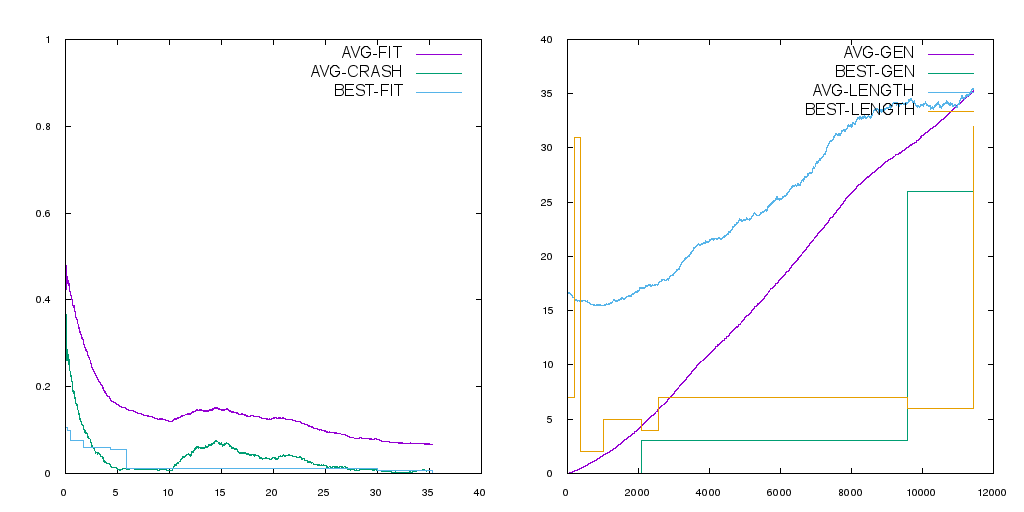
\includegraphics[width=\columnwidth]{examples/shellpattern/shellpattern.png}
  \caption{Evolving a shell-spawning chain on {tomato-RT-N18U-httpd}}
  \label{shellpattern-graph}
\end{figure}

Branching to gadgets unlisted in the chain's own genome can be
seen as a dangerous and error-prone tactic to dramatically
increase the proportion of introns in the genome. Selection for
such tactics would certainly explain the tendency for the crash
rate of the population to rise -- and to rise, typically, a few
generations before the population produces a new champion. 

There has been an observable tendency, in fact, for
\textsc{roper} populations' best performers to be those that take
strange and enigmatic risks with their own control flow --
manipulating the programme counter and stack pointer directly,
pushing values to their own call stack, branching wildly into
unexplored regions of memory space, and so on. These are traits
that we rarely see in mediocre specimens, but which are common in
chains that are either complete disasters, or which are the
population's fittest specimens. 

Such traits are even more common when we turn to a more complex
and nuanced problem set, and charge \textsc{roper} with the task
of evolving \textsc{rop}-chain classifiers -- exploits that
exhibit subtle, adaptive behaviour. 

\subsection{Classification of the Iris dataset}
%% start generating graphs for these. have the graph script also
% output latex, please. 
\textsc{Roper}'s pattern-matching capabilities allow it to
automate tasks commonly undertaken
by human hackers. The end result may not \emph{resemble} a
\textsc{rop}-chain assembled by human hands (or even by a
deterministic compiler), but its function is essentially the same
as the ones carried out by most human-crafted \textsc{rop}-chains:
to prepare the \textsc{cpu} context for this or that system call,
so that we can spawn a shell, open a socket, write to a file,
dump a region of memory, etc.  In this domain,
\textsc{roper} is not alone -- several other tools exist for
automating \textsc{rop}-chain construction (\S~\ref{sec:RopBackgnd}). 

In this section, we'll see that \textsc{roper} is also capable of
evolving chains that are, in both form and function, entirely
unlike anything designed by a human. Though it is still in its
early stages, and its achievements so far should be framed only
as proofs of concept, \textsc{roper} has already shown that it
can evolve chains that exhibit learned or adaptive behaviour. 
To illustrate this, we will set \textsc{roper} the task of
classifying Ronald Fisher and Edgar Anderson's famous \emph{Iris}
data set.%
\footnote{Available at
\url{https://archive.ics.uci.edu/ml/datasets/Iris}}
This is a fairly simple, balanced dataset, with just four
attributes, and three classes, and is widely used to
benchmark machine learning algorithms.

%%%%%%%%%%%%%
%% DETAILS %%
%%%%%%%%%%%%%

The fitness curve of our best
specimens \textit{without fitness-sharing} typically took the form of long, shallow plateaus, against the backdrop of a population swayed more by evolutionary
drift than selective pressure.  In addition, a second-order selective pressure appeared that encourages intron formation,
of which the crash rate seems to be a fairly reliable index
(crashes are the casualties of a certain method of intron
formation, in this context). This is what we see unfolding in
figure~\ref{fig:good-nosharing}. A dip in average length coincides with the peak in the crash rate, around phylogenic generation 350 -- though there is a great deal of
back-and-forth between the two curves, as if the two strategies
for intron-formation are competing.%: pad the genome with junk gadgets, or sidestep your genome by placing your bets on an extended phenotype found in the host process' memory?

\begin{figure}
  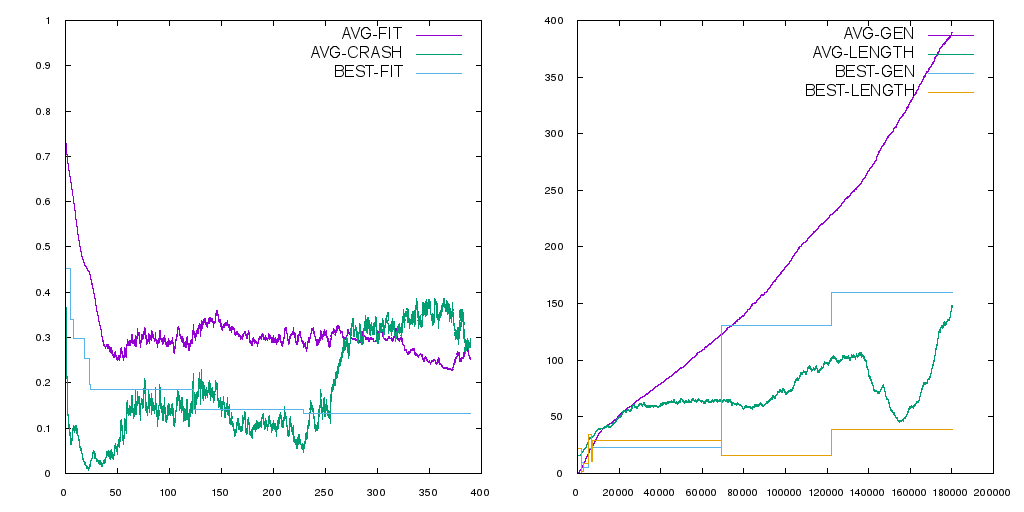
\includegraphics[width=\columnwidth]{examples/iris/good-nosharing/good-nosharing.png}
  \caption{ROPER's classification of the Iris data set, without
  fitness sharing: 86.8\,\% detection rate, after 180800
  tournaments}
  \label{fig:good-nosharing}
\end{figure}

\begin{figure}
  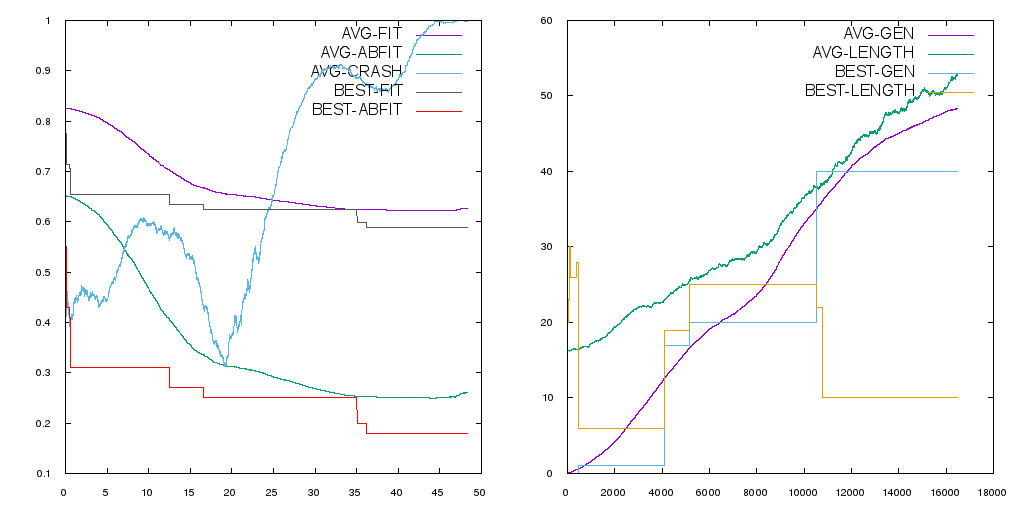
\includegraphics[width=\columnwidth]{examples/iris/plague/plague.png}
  \caption{A plague of segfaults: an overly lax crash penalty
  gives way to a 100\,\% crash rate, during ROPER's Iris
  classification. {AB-FIT} is absolute fitness,
  FIT denotes relative or shared fitness.}
  \label{fig:plague}
\end{figure}

Figure~\ref{fig:plague} shows the results of an early attempt at
implementing \textit{fitness sharing}. Here, we had factored the crash
penalties into the raw fitness passed to the sharing formula,
instead of applying them after the fact. We also overlooked a
loophole that would reduce the penalty for crashing to near zero,
so long as the return counter approached the number of gadgets
expected. There is, however, a serious vulnerability in our
implementation of the return counter. It lives in the emulator engine's
own memory space, which can be, in principle, corrupted by one of
the very \textsc{rop}-chains it is supposed to be monitoring. If
this is exploited, a specimen can artificially increment its
return counter, making it appear as if it executed its payload to
completion, while still segfaulting and raising an exception in
the virtual \textsc{cpu}. If our population was able to exploit
this feature, then it would have been able to enjoy the
protective benefits of navigating its way through a network of
deep gadgets -- resistance to destructive crossover events --
with relative ease and abandon, and no real pressure to refrain
from crashing. The result was a complete takeover of the
population by dominant, crashing genotypes: a congenital plague of
segfaults. The population was nevertheless able to achieve an 82\,\%
detection rate against Iris. 
 

Modifying the crash penalty -- making it proportional to the
prevalence of crashes in the population, a sort of segfault
thermostat -- subdued the
pressures that encouraged the population to crash, just enough to
prevent behaviour of figure~\ref{fig:plague}.
The result was a superb run -- achieving 94\,\% detection rate on
the training set in just 11,182 tournaments, 31 seasons of
difficulty rotation, and an average
phylogenic generation of just 31.9. 

\begin{figure}
  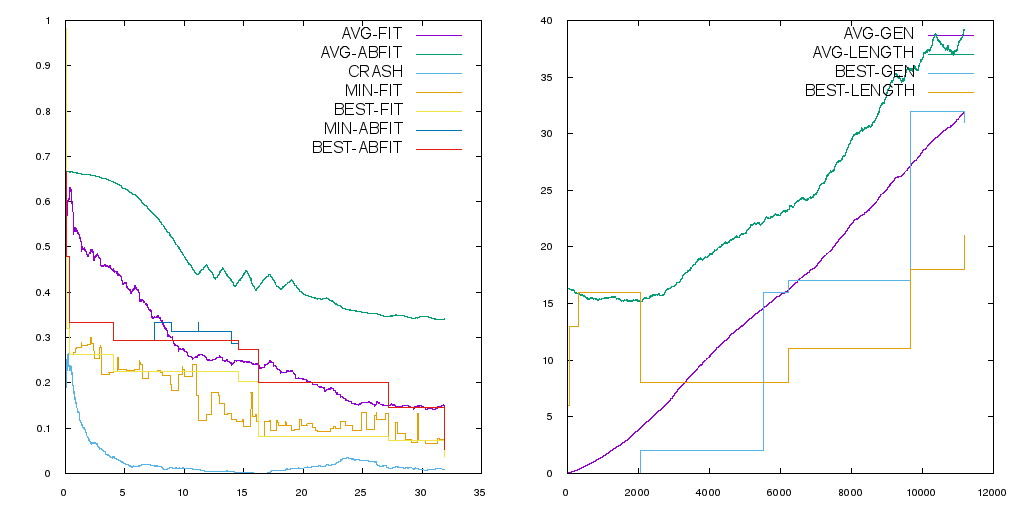
\includegraphics[width=\columnwidth]{examples/iris/sharing2/sharing2.png}
  \caption{Fitness-sharing on the Iris data set: 96.6\,\% detection
  rate on training set after just 9040 tournaments}
  \label{fig:okay}
\end{figure}

\section{Conclusion}\label{sec:conclude}

We demonstrate that return-oriented programming is a
domain in which genetic programming can be naturally and
effectively applied. Most of the techniques from
linear genetic programming can be transferred to \textsc{rop} in
a straightforward fashion. This confluence is of extreme interest
for matters of information security. It brings a host of powerful
evolutionary techniques to bear on a prevalent and persistent
mode of exploit development.%

That we are able to classify the Iris dataset is not, in
itself, remarkable. What is interesting is that this is, to our
knowledge, the first time such a thing has been carried out with
\textsc{rop}-chains -- not because there is any
sort of demand for clandestine, \textsc{dep}-subverting
flower-sorters, but because of what it shows is possible:
attacks that introduce no foreign code into a process, which
cannot be stopped by means of restrictive memory access
permissions, and which are capable of adapting to their
environment in intelligent and subtle ways, responding to cues
that may lie far beneath any human's threshold of detection, and
for which hand-coded solutions will always be too rigid and
clumsy.% With these parlour tricks \textsc{roper} has made the first, stumbling forays into an alien sphere of exploitation. 

A problem for which \textsc{roper} would be particularly
well-suited, and which we hope to explore in future work, is to
train our system to evade the detection of intelligent
\textsc{rop}-detectors like HadROP \cite{pfaff15},  
-- with the possibility of sparking a coevolutionary
arms-race that would accelerate the development and detection of
attacks. 

\begin{acks}
This research is supported by Raytheon SAS\@. The research is conducted as part of the Dalhousie NIMS Lab at: \url{https://projects.cs.dal.ca/projectx/.}
\end{acks}
